% Beamer Presentation Template
% Author: Primal Pappachan
% Last Updated: 4 - 10 - 2011
% 

\documentclass[compress,red]{beamer} %

\usetheme{Warsaw}
% other themes: AnnArbor, Antibes, Bergen, Berkeley, Berlin, Boadilla, boxes, CambridgeUS, Copenhagen, Darmstadt, default, Dresden, Frankfurt, Goettingen,
% Hannover, Ilmenau, JuanLesPins, Luebeck, Madrid, Maloe, Marburg, Montpellier, PaloAlto, Pittsburg, Rochester, Singapore, Szeged, classic

\usepackage[latin1]{inputenc}
\usefonttheme{professionalfonts}
\PassOptionsToPackage{pdftex,usenames,dvipsnames}{xcolor}
\usepackage{times}
\usepackage{tikz}
\usepackage{amsmath}
\usepackage{verbatim}
\usepackage{url}
\usepackage{graphicx}
\usepackage{graphics}

%\usecolortheme{default}
% color themes: albatross, beaver, beetle, crane, default, dolphin, dov, fly, lily, orchid, rose, seagull, seahorse, sidebartab, structure, whale, wolverine

\useoutertheme[subsection=false]{smoothbars}

\usefonttheme[onlysmall]{structurebold}

% font themes: default, professionalfonts, serif, structurebold, structureitalicserif, structuresmallcapsserif

\setbeamerfont{title}{shape=\itshape,fa mily=\rmfamily}
%\setbeamercolor{title}{fg=black!80!black,bg=red!90!white}

\logo{} %\logo{
\includegraphics[height=0.5cm]{logo.pdf}}
%% Use \insertlogo to insert the logo at place

\title{FOSSEE}
\subtitle{Pythonizing the Indian Engineering Education}
\author[]{Primal Pappachan, Parth Buch}  %\author[Euclid]{Euclid of Alexandria
\institute{IIT Bombay}
\date[]{} %\date[ISPN ’80]{27th International Symposium of Prime Numbers}

\AtBeginSection[]
{
  \begin{frame}<beamer>
    \frametitle{Outline}
    \tableofcontents[currentsection]
  \end{frame}
}


\begin{document}

\begin{frame}
	 \titlepage
\end{frame}

\begin{frame}
\section*{Outline}
\tableofcontents
\end{frame}

\section{FOSSEE}
\begin{frame}
\frametitle{FOSS for EE}
\centering{
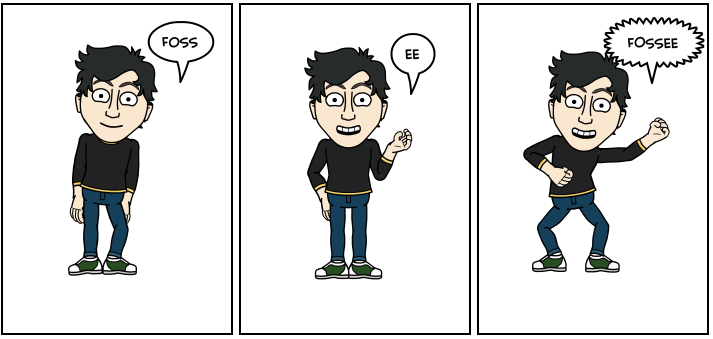
\includegraphics[scale=0.30]{foss_ee.png}
}
\end{frame}

\subsection{How}
\begin{frame}
\frametitle{How?}
\begin{itemize}
\item Improve Levels of education in India
\item Outlay of US \$ 1 Billion
\item Implemented through Information and Communication Technologies(ICT)
\item Should satisfy the requirements to be funded through the mission
\end{itemize}
\end{frame}


\begin{frame}
\frametitle{Open Source Software Creation}
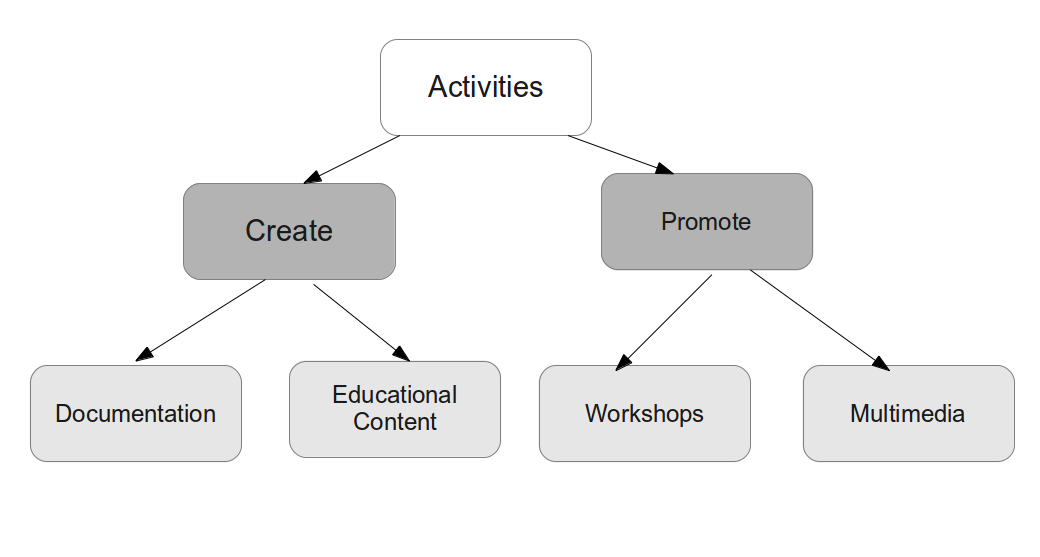
\includegraphics[scale=.30]{tree.png}
\end{frame}

\subsection{What}
\begin{frame}
\frametitle{WtF: What the FOSSEE}
\begin{block}{FOSSEE}
is  part of the National Mission on Education through ICT with the thrust area being \alert{Adaptation and deployment of open source simulation packages equivalent to proprietary software}, funded by MHRD.
\end{block}
\begin{block}{When and where}
\begin{itemize}
\item 2009
\item Based at Indian Insitute of Technology(IIT), Bombay 
\end{itemize}
\end{block}
\end{frame}

\subsection{Why}
\begin{frame}
\frametitle{Why}
\begin{columns}
\column{.5\textwidth}
\begin{exampleblock}{}
Goal of the Project
\end{exampleblock}
\column{.5\textwidth}
\begin{exampleblock}<2->{}
\begin{itemize}
\item Enable and motivate students
\item Create an innovative learning environment
\item Improving quality of learning
\item Allowing freedom in education
\end{itemize}
\end{exampleblock}
\end{columns}
\end{frame}

\begin{frame}
\begin{columns}
\column{.5\textwidth}
\begin{exampleblock}{}
In FOSS terms
\end{exampleblock}
\column{.5\textwidth}
\begin{exampleblock}<2->{}
\begin{itemize}
\item Promote 
\item Create Documentation
\item Spread Awareness
\end{itemize}
\end{exampleblock}
\end{columns}
\end{frame}


\begin{frame}
\begin{columns}
\column{.5\textwidth}
\begin{exampleblock}{}
In Python terms
\end{exampleblock}
\column{.5\textwidth}
\begin{exampleblock}<2->{}
\begin{itemize}
\item Promote 
\item Get Python into curriculum
\item Generate user support
\end{itemize}
\end{exampleblock}
\end{columns}
\begin{block}<3->{Focus}
\begin{itemize}
\item Python
\item NumPy
\item SciPy
\item Sage
\end{itemize}
\end{block}

\end{frame}



\section{SDES}
\subsection{Project Details}
\begin{frame}
\frametitle{SDES}
\begin{block}{Software Development techniques for Engineers \& Scientists}
A semster long foundation course for NON-IT Students.
\end{block}
\end{frame}

\subsection{Goals}
\begin{frame}
\frametitle{Goals}
\begin{itemize}
\item To use computer as a tool.
\item Learn how to collobrate.
\item Introduce Open Source softwares and tools.
\item Understand the importance of standards and conventions.
\end{itemize}
\end{frame}


\subsection{Content}
\begin{frame}
\frametitle{Course Content}
\begin{itemize}
\item ULT
\item Python
    \begin{itemize}
        \item Advance
            \begin{itemize}
                \item Matplotlib
                \item NumPy
                \item SciPy
            \end{itemize}
        \item Basic
            \begin{itemize}
                \item IPython
                \item DataTypes
                \item Built-in-functions
            \end{itemize}
        \end{itemize}
        \item Version Control(Mercurial)
        \item Test Driven Development
            \begin{itemize}
                \item doctest
                \item unittest
                \item nose test
            \end{itemize}
        \item LaTeX
    \end{itemize}
\end{frame}


\subsection{Reach}
\begin{frame}
\frametitle{Reach}
\begin{itemize}
\item Introduced into IIT Bombay curriculam from 2011
\item Partially introduced in BHU - Varanasi Curriculam
\item Partially introduced in BMS - Bangalore
\item 725 Teachers from across India were trained to deliver this course.
\end{itemize}
\end{frame}

\subsection{Future}
\begin{frame}
\frametitle{Future}
\begin{itemize}
\item Push this course across universities
\item Convert the courseware to Spoken Tutorials for self learning
\end{itemize}
\end{frame}

\section{Spoken Tutorials}
\subsection{Before}
\begin{frame}
\frametitle{Offline Workshops}
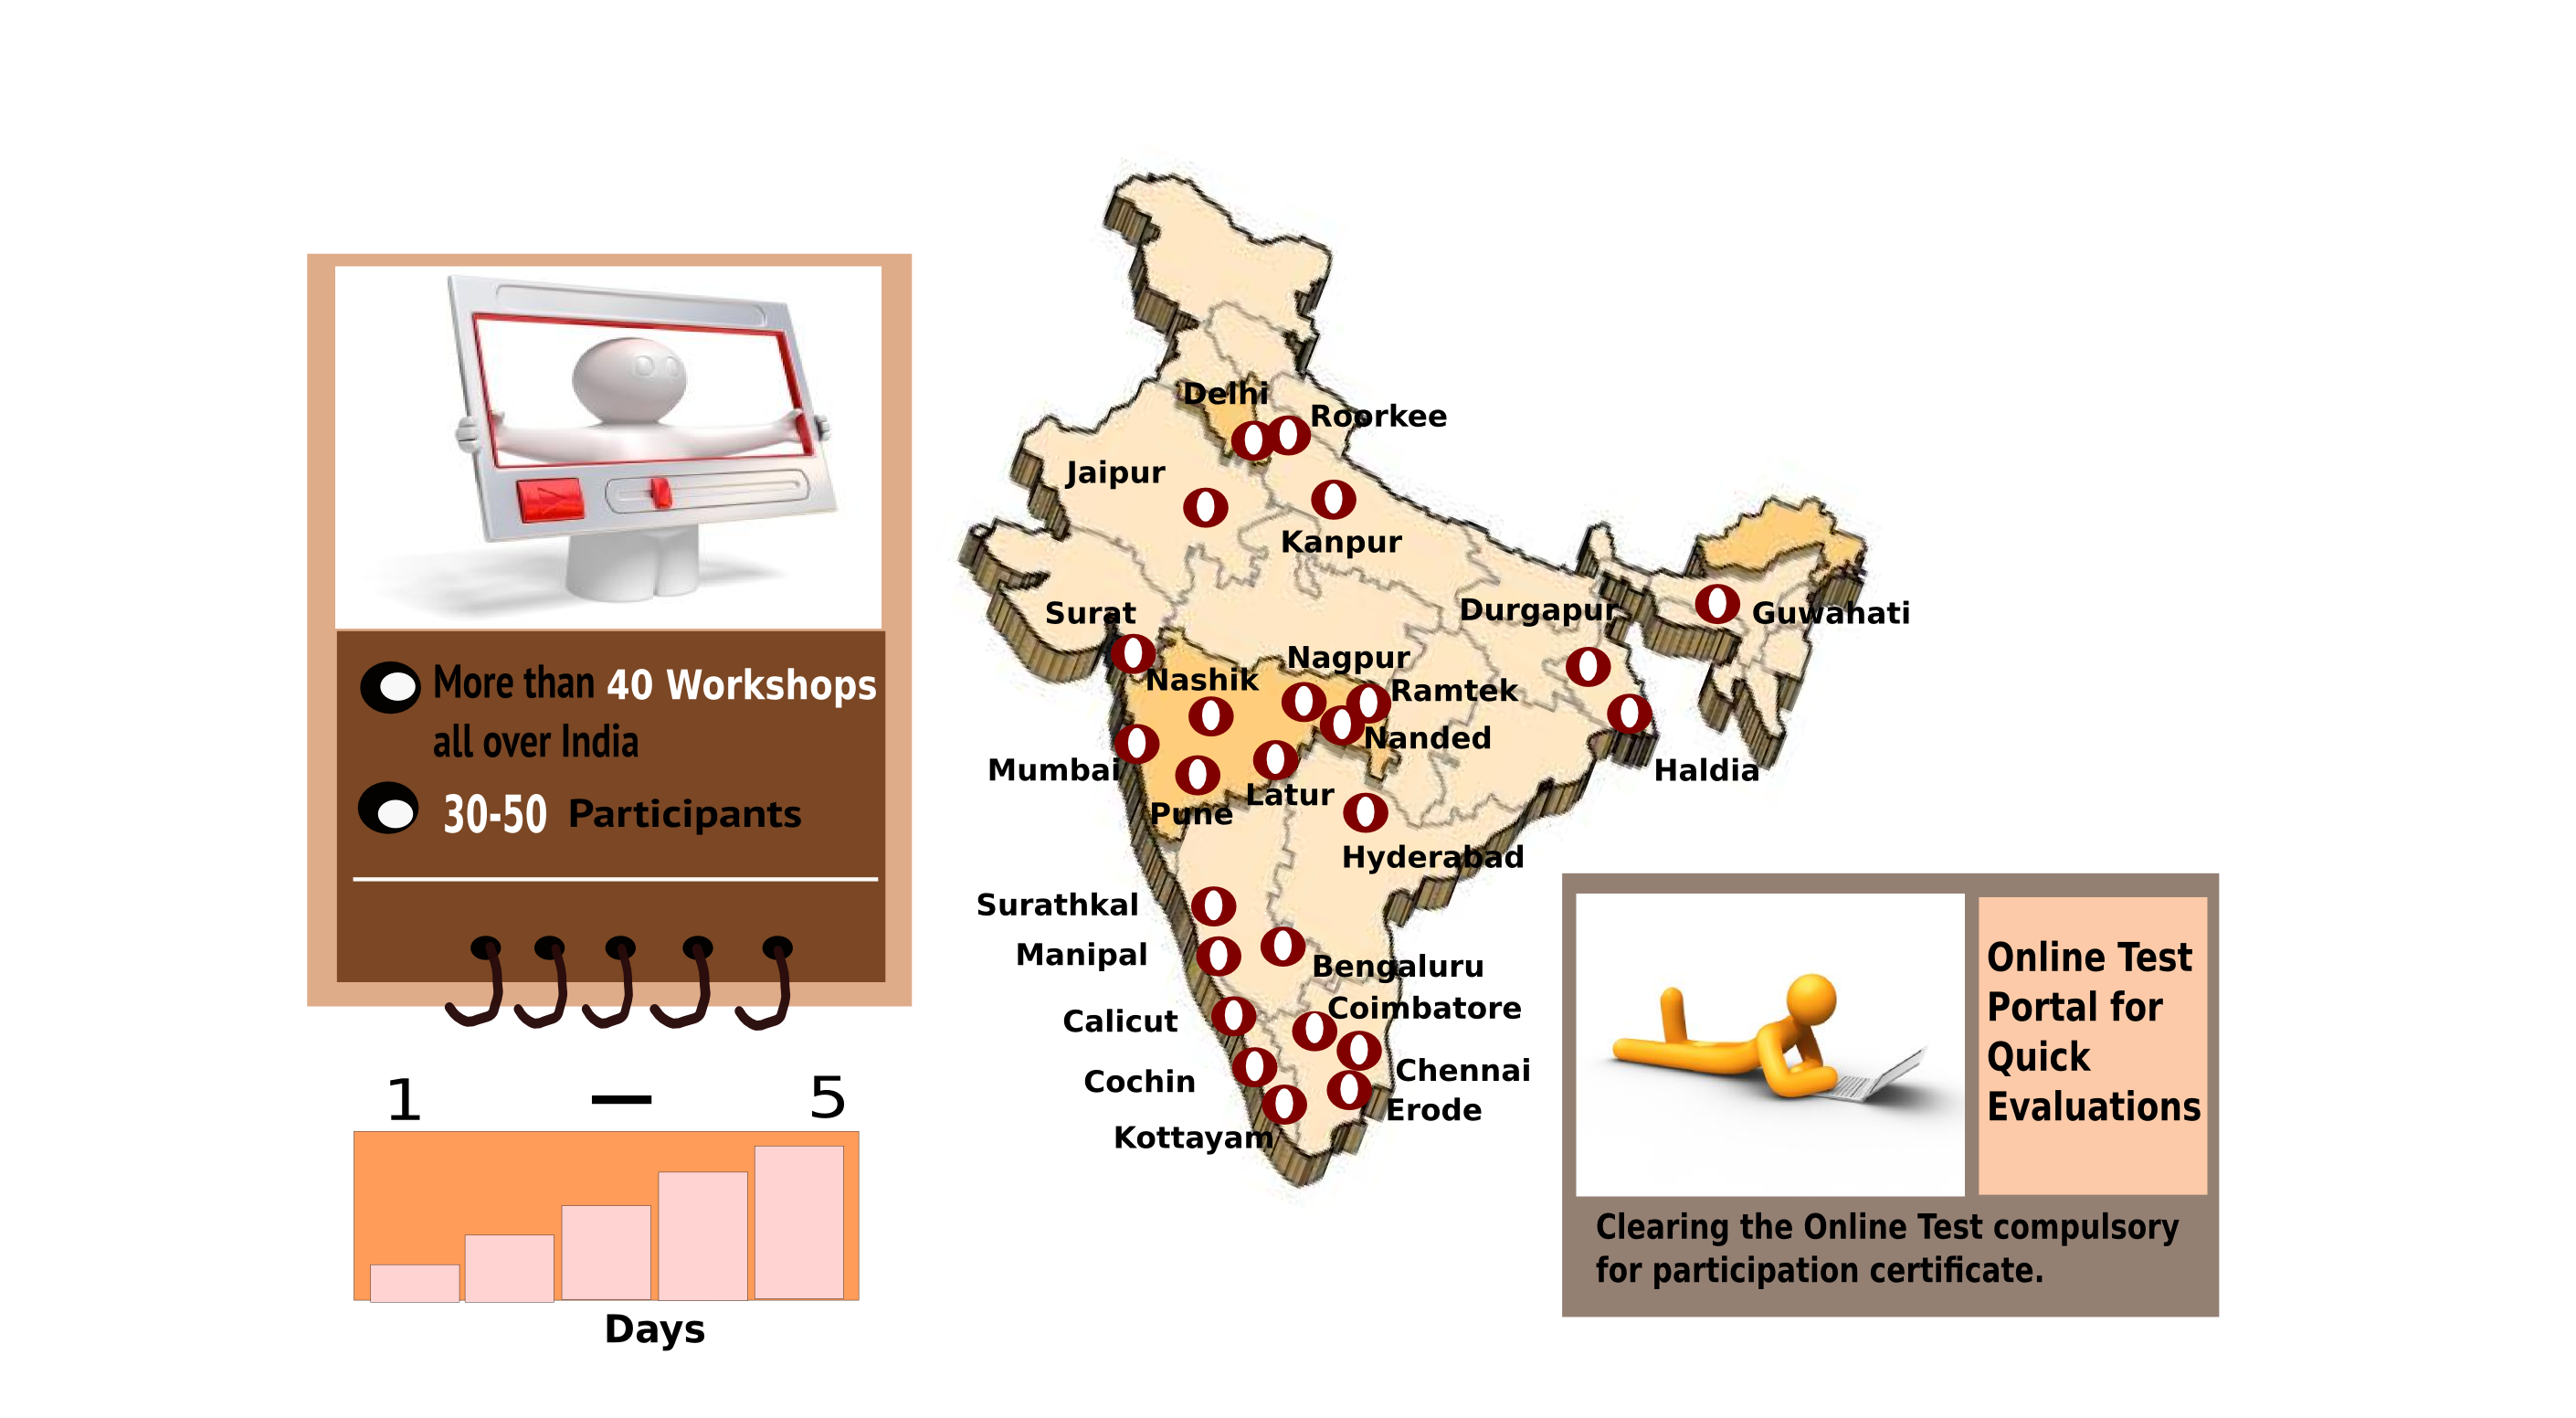
\includegraphics[scale=.15]{workshop.png}
\end{frame}

\begin{frame}
\frametitle{Limitation of Offline Workshops}
\begin{itemize}
\item Limited number of resource persons
\item Cannot be at more than one place than once
\item Expensive and time consuming
\item Knowledge fatigue and no sustained interest
\end{itemize}
\end{frame}

\subsection{After}
\begin{frame}
\begin{block}{Spoken Tutorials}
Screencasts with a running commentary which explains some aspect of a software.
\end{block}
\begin{exampleblock}{}
\begin{itemize}
\item Emphasizes Self Learning
\item Short and sweet
\item Simultaneous
\item Cost effective
\item Resusable effort
\end{itemize}
\end{exampleblock}
\end{frame}

\subsection{The Creation Process}
\begin{frame}
\begin{columns}
\column{.2\textwidth}
\column{.8\textwidth}
\frametitle{Inception to Conclusion}
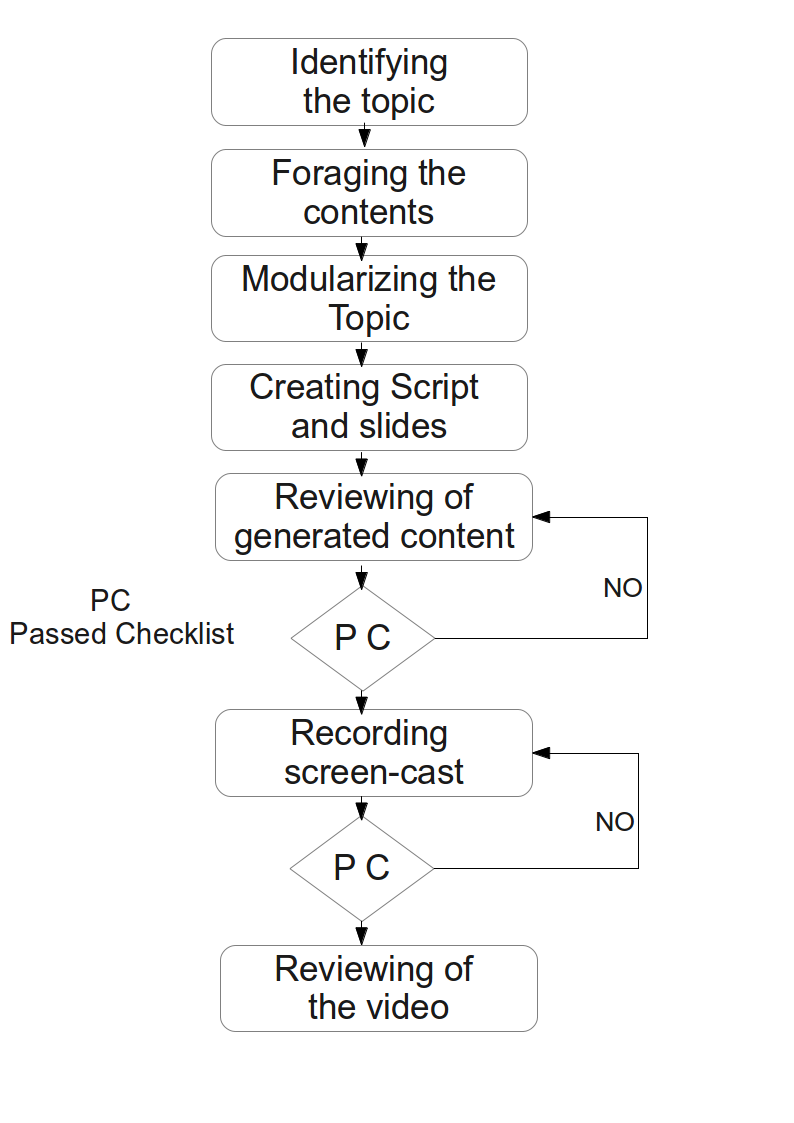
\includegraphics[scale=0.25]{st-fc.png}
\end{columns}
\end{frame}

\begin{frame}
\frametitle{1234}
\begin{itemize}
\item Topic selected based on the reachable audience
\item Content collected and modularized with the help of domain experts.
\item Creation of script with examples and evaluation questions
\item Coordination through github
\item Have to get yes for a percentage of questions on the checklist
\item Iterative process of reviewing and editing
\end{itemize}
\end{frame}

\begin{frame}
\frametitle{Recording process and Final check}
\begin{itemize}
\item Recording done after passing the first half of checklist
\item Video reviewed against the checklist
\item Novice check
\item Iterative process until it meets the requirements
\end{itemize}
\end{frame}

\subsection{Present and Future}
\begin{frame}
\frametitle{}
\begin{columns}
\column{.5\textwidth}
\begin{block}{Created}
\begin{itemize}
\item Python(Basic/Advanced)
\item Version Control
\item Linux tools
\item Test Driven Development
\item Latex
\end{itemize}
\end{block}
\column{.5\textwidth}
\begin{block}{Future topics}
\begin{itemize}
\item Machine Learning using scikits.learn
\item Image processing using scikits.image
\item Django
\item Mayavi
\end{itemize}
\end{block}
\end{columns}
\end{frame}

\begin{frame}
\frametitle{Spoken Tutorial(ST) application}
\begin{itemize}
\item User Profiling
\item Video viewing
\item Metrics for evaluating effectiveness
\item Better platform for Spoken Tutorials
\end{itemize}
\end{frame}

\begin{frame}
\frametitle{Yes, you can help}
\begin{itemize}
\item Give Novice/Expert Feedback on the videos
\item Suggest topics to be covered
\item Mention resources for content generation
\end{itemize}
\begin{block}{Achievements}
\begin{itemize}
\item 37 videos completed
\item 20 under progress
\item Over 200 workshops in last one year
\item Better reach and promotion of Python and FOSS
\item Accessible anywhere, anytime and free of cost
\end{itemize}
\end{block}
\end{frame}

\section*{}
\frame{
    \begin{center}
        \huge
        Thank you\\ \pause
    \end{center}
}

\end{document} 
